\chapter{Implementation \label{implementation}}
In design \autoref{design} all required techniques and tools were addressed and in this chapter the solution is documented. The design system is a deception technology monitoring the activity of present users or processes. Each section describes used technology, sub-problem solutions and possible changes in comparison to the designed solution. To begin with, almost all configuration and provisioning operations are covered by Ansible roles and playbooks (see~\autoref{appendix:ansible:structure}) and properly maintained (\ref{iso.12.5}) in case a needed rollback.

\section{Kubernetes \label{implementation:k8s}}
The cluster is hosted on VMs sharing a common host machine, which meets certain specifications outlined in \autoref{design:specs}. The base system consists of four VMs (see~\autoref{image:design:k8s}), each serving its purpose in the Kubernetes cluster. Precisely, there are three cluster nodes with one additional VM serving a data node.

\subsection{Deployment \label{implementation:k8s:deploy}}
%To meet the requirements 
The Vagrantfile is partially configurable via environment variables specified in extra \textit{environment.rb} (see~\autoref{listing:vagrant:environment}) file located in the same directory. Even though, they are environment variables, they inclusion in a separate ruby file is necessary.

\begin{lstlisting}[language=bash, style=custom, caption={Contents of the \textit{environment.rb}. These all available variables to configure a new deployment in different environment. Applying these variables, Vagrant create four (one master, two worker and one data node) based on \textit{generic/ubuntu1804} box. Furthermore connects each node to \textit{mybr0} network bridge and sequentially assigns IP addresses and hostnames based on the \texttt{172.30.0.0/24} network and \texttt{k8s-host.local} higher level domain respectively.}, label=listing:vagrant:environment]
# mandatory 
K8S_NETWORK_BRIDGE_NAME = "mybr0"
K8S_NODES_NET_PREFIX = "172.30.0."  # string prefix representation of 172.30.0.0/24
K8S_DOMAIN = "k8s-host.local"
K8S_SSH_PUBLIC_KEY_PATH = "~/.ssh/id_vagrant_k8s.pub"

# optional with default value
K8S_BOX_DISTRO = "generic/ubuntu1804"
K8S_MASTER_NODE_COUNT = 1
K8S_WORKER_NODE_COUNT = 2
K8S_DATA_NODE_COUNT = 1
\end{lstlisting}

The dependencies are the existence of the SSH public key, the network bridge and its IP address corresponding the prefix. The Ansible playbook \textit{vagrant\_k8s\_up.yml} prepares the dependencies, configures the Vagrantfile environment variables and runs \texttt{vagrant up}. At any point the base system can be halted with an opposing playbook \textit{vagrant\_k8s\_down.yml} At this point the base system is ready for Kubernetes cluster configuration utilizing \textit{kubespray} with specifically changed variables outlined in \autoref{listing:kubespray:vars}. To reproduce the procedure of installation follow the official guidance\footnote{\url{https://github.com/kubespray/kubespray/blob/master/README.md}}. With the defined configuration, kubespray setups Kubernetes with the additional \textit{helm}\footnote{\url{https://helm.sh/}} package manager for more convenient resource deployment.

\begin{lstlisting}[language=Clean, style=custom, caption={Changed variables in the created inventory. In addition to the the hosts defined in \textit{hosts.yaml} file, kubespray defaults with two master nodes for the setup of three nodes in total - this is changed to one master node.}, label=listing:kubespray:vars]
helm_enabled: true
\end{lstlisting}

\subsection{Environments \label{implementation:k8s:envs}}
A Kubernetes environment in terms of this thesis is a collection of resources within the same namespace (virtual cluster). Before deploying creating any resources there are a couple of playbooks setting up the data node, load balancer, cluster monitoring and the \texttt{kubectl} tool.

\begin{itemize}[noitemsep]
	\item \texttt{nfs.yml} -- Installs the NFS server on the data node and setups the NFS share directory.
	\item \texttt{metallb.yml} -- Deploys the MetalLB load balancer related resources to Kubernetes.
	\item \texttt{prometheus.yml} -- Setups Prometheus monitoring using the Helm package manager. A couple of arguments configure it and Grafana to retrieve an "public" IP address from the MetalLB address pool, isolate them to a separate namespace and other.
	\item \texttt{kubectl.yml} -- Completely configures the \texttt{kubectl} tool with bash auto-complete.
\end{itemize}

The environments designed and used are held is a separate git repository\footnote{\url{https://github.com/tomas321/k8s-environment-scenarios}}. The chosen applications and services are not that important and would require a whole research process, because it's dependent on the user. Even though, concentrating on vulnerable software is a convenient way of baiting an attacker.

Although, as of now, there is only one environment grouping multiple applications and services - Elasticsearch with Kibana, mail server\footnote{\url{https://github.com/technicalguru/docker-mailserver/tree/master/examples/kubernetes}}, git service Gitea and a custom vulnerable SSH service (vulnerable-ssh). Although, at the time of writing, not all applications are functional. The environment is meant to be versatile to mimic a production system.

For the sake of a proof-of-concept (PoC) vulnerable-ssh is the most important Pod configured with OpenSSH \textit{6.6p1-2ubuntu2.13} and most importantly Bash \textit{4.3.0(1)-release}. As such, the whole environment is considered vulnerable to the shellshock attack exploiting a Bash vulnerability (CVE-2014-6271 \cite{cve:shellshock}) and leading the attacker to run arbitrary code. This is build as a docker container on Docker Hub\footnote{\url{https://hub.docker.com/repository/docker/tbellus/shellshockable}}.

\section{Container monitoring \label{implementation:mon}}


\subsection{Reconnaissance \label{implementation:mon:recon}}
While gathering information of the system dynamically, a set od Bash scripts creates a necessary map of all the container in the environment. A collection tool \textit{sneakpeek}\footnote{\url{https://github.com/tomas321/sneakpeek}} queries the Kubernetes and Docker API, process information and setups the some of the monitoring features.

\begin{itemize}[noitemsep]
	\item \texttt{sneakpeek.sh} -- Main script calling sequentially all other scripts. It operates in two main options. \textit{fswatch} for setting up the file system monitoring as systemd services based on the "merged directory" of the docker container. \textit{procmon} for setting up the process execution monitoring with container segregation via BPF maps holding the mount namespaces. \textit{tcptracer}, similar to the latter for setting up the network connection monitoring in the same manner as \textit{procmon} option.
	\item \texttt{get\_all\_containers.sh} -- Maps the node IP address to the Docker container and returns it as comma-separated lines.
	\item \texttt{get\_container\_ns.sh} -- It is executed on each node and essentially retrieves the mount namespace of each container. (see~\autoref{listing:sneakpeek:mntns}).
	\item \texttt{bpftool\_map\_container\_ns.sh} -- It manages the creation of BPF maps holding the mount namespaces and starts the process monitoring \textit{systemd} services.
\end{itemize}

\begin{lstlisting}[language=bash, style=custom, caption={The main piece of script code for retrieving the muont namespace inode number of the given container. This is executed for each container on a corresponding node.}, label=listing:sneakpeek:mntns]
pid=$(sudo docker inspect $CONTAINER | jq -r '.[0].State.Pid');
echo $(sudo stat -Lc '%i' /proc/$pid/ns/mnt)
\end{lstlisting}

In the first iteration of development the prime script \texttt{get\_all\_containers.sh} was slowing down the whole execution due to iterating through all cluster nodes and executing programs over SSH protocol. \autoref{listing:sneakpeek:timing} shows that the improved version was 40 times faster.

\begin{lstlisting}[language=bash, label=listing:sneakpeek:timing]
sneakpeek$ time ./get_all_containers.sh 1>/dev/null

real    0m0,404s
user    0m0,163s
sys     0m0,035s
sneakpeek$ time ./get_all_containers.sh.old 1>/dev/null

real    0m16,896s
user    0m1,695s
sys     0m0,402s
\end{lstlisting}

\subsection{Threat hunting \label{implementation:mon:hunting}}
% TODO: add network monitoring
Visibility and control is vital to successfully threat hunt a occurring attack. Additional tools are deployed to monitor the process execution, networking and FS changes. Namely the \texttt{execsnoop} syscall spying tool, \texttt{tcptracer} and \texttt{fswatch} respectively. Fswatch is a forked\footnote{\url{https://github.com/tomas321/fswatch}} Github project and additionally modified to meet the requirements. Execsnoop and tcptracer are ready to use tools form the BCC dependent on the latest kernel version.

\subsubsection*{Fswatch \label{implementation:mon:hunting:fswatch}}
The existing project is functional as is. Although changing the timestamp precision and file event exclusion feature was necessary. Since it's working with \textit{sys/inotify} library, the shortest unit of time is a second. So the precision change is only in the fswatch application layer. It required a thorough inspection of the whole source code to cover each timestamp usage.

Fswatch knows and differentiates FS events. Although, a feature to exclude some events from all the whole selection was missing. The necessity was due to better readability of various usage scenarios when the requested events differ and this speeds up the process.

\begin{lstlisting}[language=bash, style=custom, caption={}, label=listing:fswatch:cmd]
fswatch --ex-event=IsSymLink --ex-event=IsDir --ex-event=IsFile --ex-event=PlatformSpecific -l 0.5 -r -x -t -f "%m-%d-%Y  %T" $DIR

# example output triggered after:
# `echo "Almost there" > $DIR/tmp/flag`
05-12-2021  16:31:07.816426 $DIR/tmp/flag Created
05-12-2021  16:31:07.816494 $DIR/tmp/flag Updated
\end{lstlisting}
\autoref{listing:fswatch:cmd} shows the command arguments used for each instance of FS monitoring process. As mentioned before, here four of 14 known events are ignored using the \textit{--ex-event} option, because they produce too many uninteresting events triggered by common programs e.g. \texttt{ls}. To not drain the CPU a latency of maximum 0.5 seconds is chosen and followed by recursive (\texttt{-r}) \textit{\$DIR} directory monitoring. Output-related flags are for including the event identifier (\texttt{-x}), timestamp of occurrence (\texttt{-t}) with a specific format (\texttt{-f "\%m-\%d-\%Y  \%T"}).

\subsubsection*{Execsnoop \label{implementation:mon:hunting:execsnoop}}
% explain the usage and the creation of the bpf map
% maybe not mention its from the official docs
Each execsnoop instance is operating in a specified mount namespace shared over a BPF map. This is ensured by the \texttt{bpftool} backed by the latest kernel. \autoref{listing:bpftool:snippet} is a \texttt{bpftool\_map\_container\_ns.sh} script snippet for creating the BPF map (mapped to a specific file typically in \textit{/sys/fs/bpf} directory) if not present already and updates it with a the mount namespace. Additionally, it starts the templated (see~\autoref{listing:systemd:execsnoop}) execsnoop systemd services.

\begin{lstlisting}[language=bash, style=custom, caption={Setup of BPF map for sharing the mount namespave with execsnoop instance. INODE variable is retrieved using the command sequence specified in \autoref{listing:sneakpeek:mntns}.}, label=listing:bpftool:snippet]
FILE=/sys/fs/bpf/mnt_ns_container1
NAME="${FILE##*/}"
NS_ID_HEX="$(printf '%016x' $INODE | sed 's/.\{2\}/&\n/g' | tac | tr '\n' ' ')"

# check if eBPF map already exists
bpfmap=$(sudo bpftool map show pinned $FILE 2>/dev/null)
if [ $? -eq 0 ]; then
  id=$(echo $bpfmap | cut -d: -f1)
  sudo bpftool map dump id $id | grep -q -i "$NS_ID_HEX"
  if [ $? -eq 0 ]; then
    # eBPF map already exists
    sudo systemctl start execsnoop@$NAME; exit 0
  fi
else
  # creating eBPF map '$FILE'
  sudo bpftool map create $FILE type hash key 8 value 4 entries 128 name $NAME flags 0
fi

# updating eBPF map with inode ID '$NS_ID_HEX'
sudo bpftool map update pinned $FILE key hex $NS_ID_HEX value hex 00 00 00 00 any
\end{lstlisting}

\begin{lstlisting}[language=Clean, style=custom, caption={Execsnoop templated systemd unit file. It executes a caller script running the execsnoop program. Program output is redirected to the local syslog server and in a custom configuration the stream is writen to file based on the "SyslogIdentifier".}, label=listing:systemd:execsnoop]
[Unit]
Description="execsnoop container %I"

[Service]
Restart=no
ExecStop=/bin/kill -9 $MAINPID
ExecStart=/usr/local/bin/sneakpeek/execsnoop_caller.sh /sys/fs/bpf/%i
StandardOutput=syslog
StandardError=syslog
SyslogIdentifier=execsnoop_%i
\end{lstlisting}

\subsubsection*{Tcptracer \label{implementation:mon:hunting:tcptracer}}
A stateful tool capturing changes in TCP connections made to and from the target system. Namely the accept, close and connect operations. It's differentiating containers by the mount namespace utilizing the same technique (see~\autoref{listing:bpftool:snippet}) as execsnoop. \autoref{image:implementation:tcptracer} shows the example output, how it copes with displaying the active connections. The down side is that it's difficult to trace the connection when analyzing the output.

\begin{figure}[h]
	\centering
	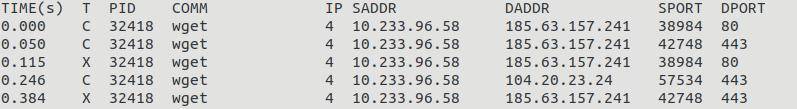
\includegraphics[scale=0.4]{tcptracer}
	\caption{Example output of the TCP tracer program.}
	\label{image:implementation:tcptracer}
\end{figure}

Each tcptracer process is started by a caller script, which in term is managed by systemd. A caller script has the advantage of high flexibility in case of pre-execution operations. Regarding systemd, tcptracer failed to log its output in the same way as for execsnoop specified in \autoref{listing:systemd:execsnoop}. A proposed and realized fix\footnote{Refer to the forked repository proposing this change - \url{https://github.com/tomas321/bcc/tree/fix/proper-tcptracer-print-function}} was to copy the same printing strategy from execsnoop.

\subsubsection*{Deployment \label{implementation:mon:hunting:deploy}}
Fswatch, tcptracer and execsnoop are deployed and configured using the combination of \texttt{sneakpeek.sh} script and Ansible playbooks.
\begin{itemize}
	\item \texttt{fswatch.yml} - Fully configures all nodes with fswatch by runnig the \texttt{sneakpeek.sh} script and ultimately starting systemd services for each container.
	\item \texttt{sneakpeek.yml} - Similarly, completely configures the nodes with process monitoring running execsnoop and network connection monitoring running tcptracer as systemd services.
\end{itemize}
All are logging their according the \ref{iso.12.4}. The attackers agenda can be identified by inspecting the logged information in the designated location - \textit{/var/log/sneakpeek}.

\subsubsection*{Management \label{implementation:mon:hunting:mgmt}}
To have control over the monitoring services running on each node, additionally the \textit{sneakctl\_server}\footnote{\url{https://github.com/tomas321/sneakctl_server/}} provides some management related features. It is implemented as a Flask REST API in abidance with \ref{iso.12.5} serving an additional access to the systemd services on nodes and increased increased visibility of processes and files on each container. Concretely, there are four main endpoint groups - process, fswatch, execsnoop and file (see~\autoref{appendix:sneakctl}).

It introduces a faster way of management and additional look at process instances and file statistics. Essentially the fswatch and execsnoop endpoint groups are wrappers over the systemd service utilizing the \texttt{dbus} library. Process and file endpoints simple query the statistics of the provided asset - be it absolute path to a file or the process ID.

This is particularly useful, because the live monitoring data are in a stream of log lines with basic information. It safes time, which is in live system compromisation crucial.

\section{Proof of concept - experiment \label{implementation:poc}}
The experiment consists of demonstrating the introduced monitoring tools. The set environment comprises of a single custom container vulnerable to the \textit{shellshock} attack. With all the monitoring tools enabled the container is accessed via over SSH exploiting the shellshock vulnerability (see~\autoref{image:poc:exploit}).

\begin{figure}[h]
	\centering
	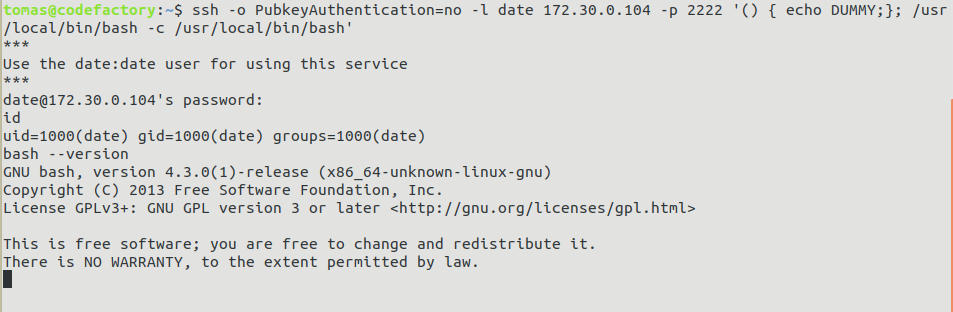
\includegraphics[scale=0.44]{shellshock_exploit}
	\caption{The 'shellshockable' container is running within Kubernetes. It's published via a \textit{LoadBalancer} Service mapping the SSH port to port \textit{TCP/2222}. The IP is dynamically assinged from an address pool to \texttt{172.30.0.104}.}
	\label{image:poc:exploit}
\end{figure}

\begin{figure}[h]
	\centering
	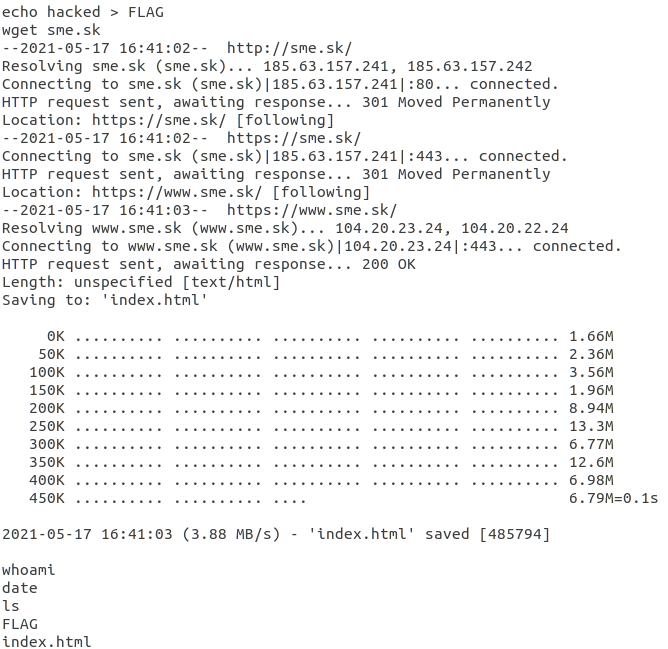
\includegraphics[scale=0.44]{shellshock_shell}
	\caption{Shell commands executed. All are then visible in the below listed screen shots}
	\label{image:poc:shell}
\end{figure}

\autoref{image:poc:shell} displays the commands executed in the non-interactive shell, which means that all input/output text is as if part of a single stream. At one point the actor downloads a file from the Internet (\texttt{sme.sk} in the example) saving it to \texttt{index.html}. In \autoref{image:poc:execsnoop}, \autoref{image:poc:tcptracer} and \autoref{image:poc:fswatch} all these executed commands are seen from a different perspective.

\begin{figure}[h]
	\centering
	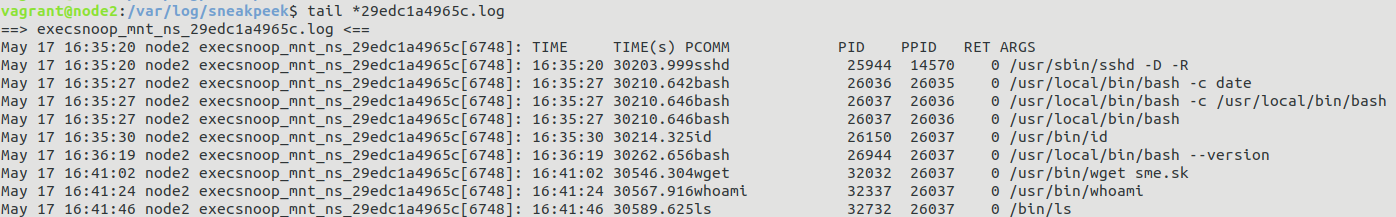
\includegraphics[scale=0.3]{poc_execsnoop}
	\caption{}
	\label{image:poc:execsnoop}
\end{figure}

\begin{figure}[h]
	\centering
	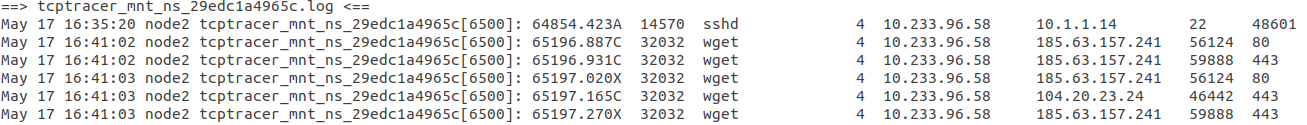
\includegraphics[scale=0.3]{poc_tcptracer}
	\caption{}
	\label{image:poc:tcptracer}
\end{figure}

\begin{figure}[h]
	\centering
	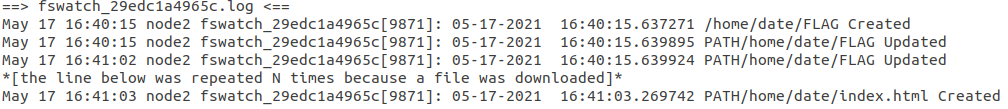
\includegraphics[scale=0.4]{poc_fswatch}
	\caption{To fit into the page the added \texttt{PATH} can be replaced by \texttt{/var/lib/docker/overlay2/LONG\_ID/merged}.}
	\label{image:poc:fswatch}
\end{figure}

Overall, all processes executed, files created and connections made are documented and it creates an image of the attacker's agenda. Even though this is only a proof of concept, in case of a more complex attack the usability is the same.

%- network traffic is monitored by tapping to the mapped interface on the host system
%1. get the docker container pid
%2. us nsenter to execute 'ip addr' to get the main net interface
%3. from that get the mapped interface 
%4. tap on that interface with tcpdump or some other software